\documentclass[a5paper,10pt,twoside,onecolumn,openany,helvetica,showtrims]{memoir}
\usepackage{tikz}
\usepackage{microtype}
\usepackage{pdfpages} 
\usepackage{lipsum}
\usepackage{float}
\restylefloat{table}
\usepackage{subcaption}
\usepackage{metalogo}
\usepackage{tabularx,url,booktabs}
\usepackage[pdfauthor={Jack J. Miller}, unicode,plainpages=false,pdfpagelabels,colorlinks=false,hidelinks]{hyperref}
\hypersetup{colorlinks=false,bookmarksdepth=2}

%Sans serif fonts
\renewcommand{\familydefault}{\sfdefault}

%Paper trims and bleeds for the printer 

\setstocksize{225mm}{160mm} %SRA5 
\settrimmedsize{210mm}{148mm}{*} %A5 
\setlength{\trimtop}{\stockheight} % \trimtop = \stockheight
\addtolength{\trimtop}{-\paperheight} % - \paperheight
\setlength{\trimedge}{\stockwidth} % \trimedge = \stockwidth
\addtolength{\trimedge}{-\paperwidth} % - \paperwidth
\settrims{0.5\trimtop}{\trimedge}
\quarkmarks %at their request

% Uncomment the below to hide crop marks automatically -- but we need to change the numbers to be the crop dimensions in bp. 


%\usepackage{atbegshi}
%\AtBeginShipout{\special{pdf: put @thispage <</TrimBox [36.0 36.0 612 810]>>}}
%\special{pdf: put @thispage <</TrimBox [36.0 36.0 612 810]>>}

\isopage %as opposed to \medievalpage. 

%Memoir commands 
\setlrmarginsandblock{11mm}{12mm}{*} %1mm gutter should be enough for a thin book 
\setulmarginsandblock{17mm}{*}{1}
\setheadfoot{8pt}{20pt}
\checkandfixthelayout


%Hide large CHAPTER 1 in headings 
\addtopsmarks{headings}{}{
  \createmark{chapter}{left}{nonumber}{}{}
}

\pagestyle{headings} % activate changes
\nouppercaseheads %Make title case 
\copypagestyle{jackheading}{headings}%Duplicate existing style to edit it 

\makeevenhead{jackheading}{\thepage}{}{}
\makeoddhead{jackheading}{}{}{\leftmark \quad \thepage}

\pagestyle{jackheading}%activate
%%%%%%%%%%%%%%%%%%%%%%%%%%%%%%%%%%
% Chapter styling
\makechapterstyle{jackdemo}{
\chapterstyle{demo}
   \setlength{\beforechapskip}{-2cm}     % corrected command \midchapskip to \beforechapskip
   \setlength{\afterchapskip}{2.5cm}
    \renewcommand{\printchaptername}{}
    \renewcommand{\printchapternum}{\hspace*{\textheight}}
}



% Below lengths are for the conference programme
\newlength{\JackBoxOne}
\setlength{\JackBoxOne}{0.1395\textwidth}%originally 0.15
\newlength{\JackBoxTwo}
\setlength{\JackBoxTwo}{0.09\textwidth}%originally 0.15
\newlength{\JackBoxThree}
\setlength{\JackBoxThree}{0.65\textwidth}%originally 0.65
\newlength{\LittleSkip}
\setlength{\LittleSkip}{0.25em}
\setlength{\parindent}{0em}

%Speaker pictures 
\newlength{\SpeakerSize}
\setlength{\SpeakerSize}{0.3\textwidth}

\counterwithout{section}{chapter} %Don't show section numbers in the TOC
\global\hyphenpenalty=300 %Increase hyphenation penalty 

%%%%%%%%%%%%%%%%%%%%%%%%%%%%%%%%%
\newcommand{\talkauthor}[1]{\small\emph{#1}}
\usepackage{longtable}
\usepackage{wrapfig}
\usepackage{adwrapfig}
\usepackage{multicol}

\setsecnumdepth{chapter}

\checkandfixthelayout
\AtBeginDocument{\addtocontents{toc}{\protect\thispagestyle{empty}}} 
\begin{document}
%%%%%%%%%%%%%%%%%%%%%%%%%%%%%%%%%%%%%%%%%%%%%%%%%%%%%%%%%%%%%%%%%%%%%%%
% The coverpage "for previewer purposes" is below 
%\includepdf[pages={2}]{BackgroundImages}
\frontmatter\thispagestyle{empty}\cleartoverso%\clearpage
\checkandfixthelayout
\thispagestyle{empty} %colophon page below 
    \vspace*{\fill}
    \begin{minipage}{0.45\textwidth}
	\tiny Please recycle this booklet when you are finished with it.\\ Printed and bound in the UK on recycled acid-free paper by the Holywell Press, www.holywellpress.com. \\[2em]
	Set in Latin Modern with the \XeLaTeX{} document preparation system by Jack J. Miller and Justin Y.~C.~Lau.\\[2em]
	The source code for this document is available online at github.com/NeutralKaon/BCISMRM-Conference-Booklet. 
    \end{minipage}\cleartorecto
\tableofcontents*
\chapterstyle{jackdemo}
\mainmatter
%%%%%%%%%%%%%%%%%%%%%%%%%%%%%%%%%%%%%%%%%%%%%%%%%%%%%%%%%%%%%%%%%%
\chapter{Welcome}
On behalf of the local organising committee, it is my great pleasure to welcome you to the 24\textsuperscript{th} annual scientific meeting of the British Chapter of the International Society for Magnetic Resonance in Medicine and to the beautiful city of Oxford.  It has been great fun bringing together what we hope will be an interesting, exciting and forward looking programme. The local organising committee were in complete agreement that we wanted the meeting to be a real celebration of ``the next generation of MRI'' – both in terms of the next generation of technology and developments but also the next generation of amazing scientists presenting their work. With 36 oral presentations, 24 power pitches and 29 poster presentations it will hopefully be a meeting packed with great science. Add on top of that, some amazing invited speakers and the wonderful Joe Ackerman delivering the Bill Moore Lecture -- we should have a feast of fascinating ideas to talk about. However, it shouldn't be all work, work, work! With a murder mystery themed treasure trail around the dreaming spires, an early morning park run and a gala dinner at the delightful Somerville College -- there should be something for everyone to enjoy.\\


Welcome again, we hope you enjoy the meeting and visiting Oxford -- if you have any questions or problems – just stop one of the local organising committee -- they will be happy to try and help.\\

 
Best,\\[2em]
 

Damian.\\[3em]
\emph{\hfill Damian J. Tyler}\\
\emph{Professor of Physiological Metabolism}\\
\emph{British Heart Foundation Senior Research Fellow}\\
\emph{Tutorial Fellow in Medicine, Somerville College}
%%%%%%%%%%%%%%%%%%%%%%%%%%%%%%%%%%%%%%%%%%%%%%%%%%%%%%%%%%%%%%%%%%
% Sponsors below 
\chapter{Sponsors}
\subsection{Gold Sponsors}
\begin{center}
\vfill
\includegraphics[width=0.6\textwidth]{Sponsors/converted/bruker_logo}\\
		\vfill
		\includegraphics[width=0.6\textwidth]{Sponsors/converted/philips_logo}
	\vfill
\end{center}



\includepdf{Sponsors/pet_mr_ad_A4_print}
\includepdf[noautoscale=true, height=\paperheight]{Sponsors/PhilipsAdvert}

\subsection{Silver Sponsors}

\begin{center}
\vfill
	\includegraphics[width=0.5\textwidth]{Sponsors/converted/aspect_logo}
	\vfill
	\includegraphics[width=0.5\textwidth]{Sponsors/converted/ge_healthcare_logo} \vfill
		\includegraphics[width=0.5\textwidth]{Sponsors/converted/LTO-logo-full-RED-screen}
		\vfill \includegraphics[width=0.5\textwidth]{Sponsors/converted/mrsolutions_logo}\vfill
\includegraphics[width=0.5\textwidth]{Sponsors/converted/siemens_logo}
\vfill
\end{center}

\clearpage
\subsection{Bronze Sponsors}
\begin{center}
\vfill
		\includegraphics[width=0.45\textwidth]{Sponsors/converted/crs_logo} \hfill
		\includegraphics[width=0.45\textwidth]{Sponsors/converted/Circle_Logo} \\
	\vfill 
		\includegraphics[width=0.45\textwidth]{Sponsors/converted/perspectum_logo} \hfill
		\includegraphics[width=0.45\textwidth]{Sponsors/converted/pulseteq_logo} \\ 
	\vfill		
	\includegraphics[width=0.45\textwidth]{Sponsors/converted/rapid_logo} \hfill \includegraphics[width=0.45\textwidth]{Sponsors/converted/stratech_logo} \\ 
	\vfill
	\includegraphics[width=0.45\textwidth]{Sponsors/converted/Tesla_Logo_notext}
	\vfill
\end{center}
\clearpage
\begin{vplace}[1]
\begin{center}
\begin{minipage}{0.6\textwidth}
	\itshape We are incredibly grateful to our sponsors, who not only provide a vast array of scientific and medical equipment and services, but without whom this event would simply not be possible. \\[2em]
	
	Please visit and talk to them!
\end{minipage}
\end{center}
\end{vplace}
%%%%%%%%%%%%%%%%%%%%%%%%%%%%%%%%%%%%%%%%%%%%%%%%%%%%%%%%%%%%%%%%%%
\chapter{Information}
\vspace{-5em}
\section*{Boring but important}
We do not expect routine fire alarm tests in any of the venues during the conference, so please leave should it sound (as a continuous, loud tone) by the nearest available exit.

Regarding wireless internet access, \textbf{if you have access to eduroam} then \textbf{please use it!} It's accessible in most places in the city, including all the conference venues. We have a \emph{limited} number of guest accounts for the unencrypted wireless network OWL -- please contact a member of the committee if you require one.

Regarding dietary requirements, the catering staff at all venues have been informed ahead of time about the requirements of those attending. If that applies to you, please just have a friendly chat with them and make your requirements known. 


Do not hesitate to get in touch with the local organising committee with literally any questions about anything that you may have --- we are all more than happy to help (or just to chat!) 
\section*{Directions from Somerville}
\subsection{Workshop Monday 24\textsuperscript{th} September at the Department of Physiology Anatomy and Genetics}
To get to the Department of Physiology, Anatomy, and Genetics (Sherrington Building) for the workshop on Monday leave Somerville by the porters' lodge gate and turn right. At the traffic light cross the road left towards St.~Giles' Church. Pass the church on the left with the graveyard on your right to the next set of traffic lights and cross. Follow down Keble road, past half of Physics and Computer Science, and turn right at the end into Parks Road. At the next traffic light cross over the street and enter the Science campus via Sherrington Road. Follow the road past the other half of Physics on your left. The Sherrington reception is on your left, opposite New Biochemistry (the colourful glass building). 

\begin{figure}[H]
\centering
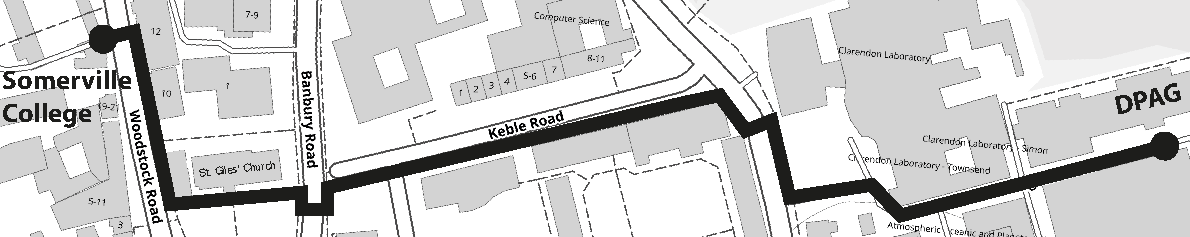
\includegraphics[width=\textwidth]{Maps-V1}
\end{figure}



\subsection{Main meeting: Tuesday/Wednesday 25\textsuperscript{th}/26\textsuperscript{th} September at the Medical Sciences Teaching Centre}
To get to the Medical Sciences Teaching Centre for the main meeting on Tuesday and Wednesday leave Somerville by the porters' lodge gate and turn right. At the traffic light cross the road left towards St Giles’ Church. Pass the church on the left with the graveyard on your right to the next set of traffic lights and cross. Follow down Keble road past half of Physics and Computer Science and turn right at the end into Parks Road. At the next traffic light cross over the street and enter the Science campus via Sherrington Road. Follow the road past the other half of Physics and observe the Sherrington Building (DPAG) on your left and New Biochemistry (colourful glass building) on your right. Follow the small pedestrian road past the Old Observatory (bending right past a 950 MHz NMR spectrometer buried underground) and then turn left onto Darlington Link. The Medical Sciences Teaching Centre (MSTC) is ahead of you through a little gate (do not follow Darlington link as it bends right). 
\begin{figure}[H]
\centering
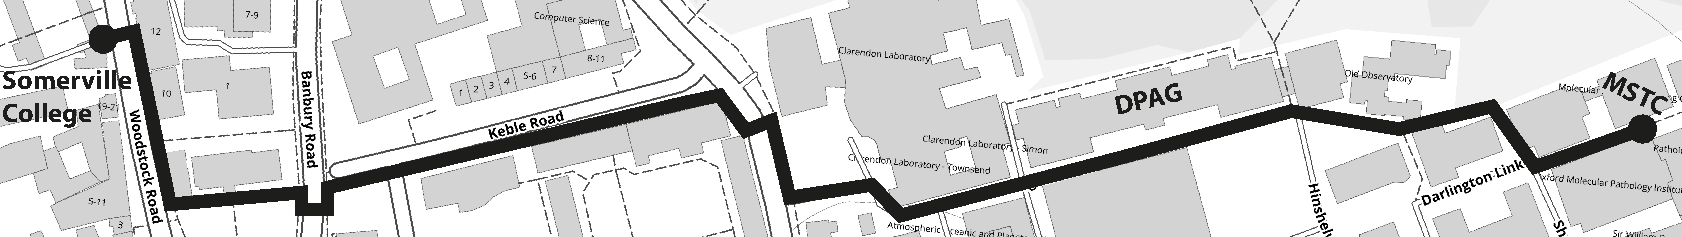
\includegraphics[width=\textwidth]{Maps-V2}
\end{figure}
\subsection{Elected pub trip to the Duke of Cambridge after the gala dinner}
To get to the Duke of Cambridge pub after the gala dinner leave Somerville by the porters' lodge gate and turn right. At the next road (Little Clarendon Street) turn right. The Duke of Cambridge is on your right between two restaurants, Carluccio's and Pierre Victoire. 

\begin{figure}[H]
\centering
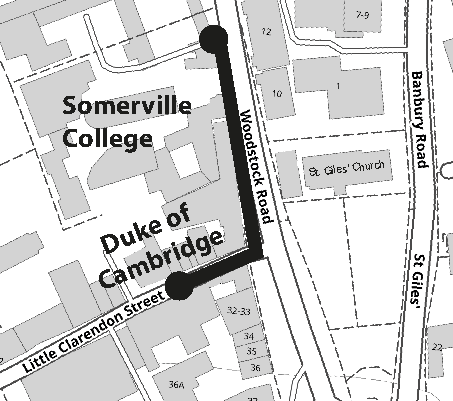
\includegraphics[width=0.4\textwidth]{Maps-V3}

\end{figure}

\section*{Acknowledgements}


The local organising committee would very much like to thank the following people for kindly giving up their time to review the abstracts submitted to the meeting:

\begin{multicols}{2}
\itshape Mark Chiew

Will Clarke

Michiel Cottaar

Sean Fitzgibbon

Ludovica Griffanti
 
Aaron Hess 
  
James Larkin

Justin Lau

Kevin Ray

Alex Smith
  
Kerstin Timm
   
Liz Tunnicliffe
    
Laci Valkovic.
\end{multicols}


We are also indebted to all the members of the local organising committee: 

\begin{multicols}{2}
\itshape Vicky Ball

Michael Chappell

Jane Francis

Yvonne Green

Peter Jezzard

Heidi Johanssen-Berg

Jack Miller

Karla Miller

Stefan Neubauer

Niki Sibson

Kerstin Timm

Damian Tyler
\end{multicols}


%%%%%%%%%%%%%%%%%%%%%%%%%%%%%%%%%%%%%%%%%%%%%%%%%%%%%%%%%%%%%%%%%%
\chapter{Programme}
\begin{center}

\textbf \emph \Huge Driving the Next Generation of MRI	
\end{center}
\vspace{5em}
\section{Monday 24\textsuperscript{th} September}
\subsection*{Workshop -- Clinical Translation of Molecular/Metabolic Imaging}
\begin{tabular}{lll}
	1300 -- 1400 & Registration&\\
	1400 -- 1430 & Invited Talk & How to do a CEST MRI Experiment \\ 
	&   & \talkauthor{Simon Walker-Samuel, University College London} \\ 
	1430 -- 1500 & Invited Talk & How to do a Hyperpolarized \textsuperscript{13}C MRI Experiment \\ 
	&	&	\talkauthor{Kerstin Timm, University of Oxford}\\
	1500 -- 1530 & \textbf{Break} & \\[\LittleSkip]
	1530 -- 1630 & Demo & Hands on demonstration sessions in two groups:  \\
				 & &  \textbullet CEST MRI \\ 
				 & & \textbullet Hyperpolarized \textsuperscript{13}C MRS \\[\LittleSkip]
	1630 -- 1700 & Invited Talk & Clinical Translation of CEST MRI\\
	& & \talkauthor{Mina Kim, University College London} \\[\LittleSkip]
	1700 -- 1730 & Invited talk & Clinical Translation of Hyperpolarized \textsuperscript{13}C MRI \\ 
	& 	& \talkauthor{Shonit Punwani, University College London} \\[\LittleSkip]
	1730 -- \emph{?} & & Murder Mystery Themed Treasure Trail 
\end{tabular}
\clearpage

\section{Tuesday 25\textsuperscript{th} September}

\noindent\hspace{-0.75em}\begin{tabular}{p{\JackBoxOne}p{\JackBoxTwo}p{\JackBoxThree}}
0830 -- 0915 & Registration & \\ 
0915 -- 0930 & Welcome & \talkauthor{Damian Tyler, University of Oxford} \\	 	
\end{tabular}
\subsection*{Session 1 -- New Horizons in MRI}
\begin{flushright}
\itshape Moderators: Penny Gowland (University of Nottingham) 

Justin Lau (University of Oxford)
\end{flushright}
\noindent\hspace{-0.75em}\begin{tabular}{p{\JackBoxOne}p{\JackBoxTwo}p{\JackBoxThree}}
0930 -- 0950 & Invited Talk & Oxygen Delivery Quantification Using Oxygen-Enhanced MRI \\ 
			& & \talkauthor{Geoffrey Parker, Manchester University} \\ 
0950 -- 1000 & O1 & Silent Myelin Imaging using Magnetization Prepared RUFIS \\ 
			 &	   & 
			 \talkauthor{Tobias Wood, King's College London} \\ 
1000 -- 1010 & O2 & Heavily Undersampled Radial Acquisition of Dynamic Vessel-Encoded Arterial Spin Labelling Angiograms Reconstructed in a Compressed Sensing Framework\\
			 &    & \talkauthor{Sophie Schauman, University of Oxford} \\ 
1010 -- 1020 & O3 & Hybrid Acquisition for Water and Adipose tissue Imaging (HAWAII)\\
			 & 	  & \talkauthor{Andreas Wetscherek, The Institute of Cancer Research} \\ 
1020 -- 1030 & O4 & Comparison of Optimized Single-PLD, Sequential and Time-Encoded Multi-PLD PCASL Methods for CBF Accuracy and Reproducibility\\
			& 	  & \talkauthor{Joseph Woods, University of Oxford} \\ 
1030 -- 1040 & O5 & Non-Invasive Imaging of CSF-Mediated Brain Clearance Pathways Via Assessment of Perivascular Fluid Movement with Diffusion Tensor MRI \\ 
			& 	&\talkauthor{Jack Wells, University College London} \\ 
1040 -- 1050 & O6 & A Whole-Body Transmit/Receive RF System for Hyperpolarized \textsuperscript{129}Xe MRI \\
			&	& \talkauthor{Claudio Puddu, University of Sheffield} \\ 
1050 -- 1100 & O7 & Microporous Lung Phantoms for 19F MRI of Inhaled Imaging Agents with Physiologically Representative Relaxation Times \\
			&	& \talkauthor{Mary Neal, Newcastle University} \\ 
1100 -- 1110 & O8 & Looping Star -- a Novel Silent Approach to Imaging Brain Function in Health and Disease \\ 
            &   & \talkauthor{Nikou Damestani, King's College London}\\
1110 -- 1140 & \textbf{Break} & 
\end{tabular}

\subsection*{Session 2 -- Machine Learning, Big Data, and Novel Analysis Techniques}
\begin{flushright}
\itshape Moderators: Karla Miller (University of Oxford)  

Sean Fitzgibbon (University of Oxford)
\end{flushright}


\noindent\hspace{-0.75em}\begin{tabular}{p{\JackBoxOne}p{\JackBoxTwo}p{\JackBoxThree}}
1140 -- 1200 & Invited Talk & Machine Learning for Cardiac MRI: Applications to Reconstruction, Super-Resolution and Analysis \\ 
		&	& \talkauthor{Daniel Rueckert, Imperial College London} \\
1200 -- 1210 & O9 & Correction of Intra-Volume Movement and Motion-by-Susceptibility
Distortion in fMRI \\ 
		&	& \talkauthor{Sean Fitzgibbon, University of Oxford}	 \\
1210 -- 1220 & O10 & Partial Volume Correction Affects Detection of Task Activation in Arterial
Spin Labelling Data \\ 
		&	& \talkauthor{Flora Kennedy McConnell, University of Oxford} \\ 
1220 -- 1230 & O11 & Automatic Classification of Benign and Malignant Prostate Lesions in
VERDICT DWMRI Using Convolutional Encoder-Decoder Architectures \\ 
		&	& \talkauthor{Eleni Chiou, University College London}\\
1230 -- 1240 & O12 & Model-Based Super-Resolution Reconstruction of T2 Maps \\ 
		&	& \talkauthor{Wajiha Bano, University of Edinburgh} \\ 
1240 -- 1250 & O13 & Classification of Type-2 Diabetes vs. Healthy Volunteers Using Features
Extracted from Cerebral Hemodynamic Signals \\ 
		&	& \talkauthor{Maria-Eleni Dounavi, University of Sheffield} \\ 
1250 -- 1300 & O14 & Fibre-to-Field Dependency of T1 Relaxation Time in Human White
 Matter at 3T \\ 
 		& 	& \talkauthor{Risto Kauppinen, University of Bristol}\\[\LittleSkip]
 1300 -- 1415 & \textbf{Lunch} & \hfill\emph{(Including mentoring event at 1345)}
\end{tabular}


\subsection*{Session 3 -- Combining MRI with Other Technologies}
\begin{flushright}
\itshape Moderators: Andrew Blamire (Newcastle University)

Po-Wah So (King's College London)
\end{flushright}
\vspace{-2em}\noindent\hspace{-0.75em}\begin{longtable}{p{\JackBoxOne}p{\JackBoxTwo}p{\JackBoxThree}}
1415 -- 1435 & Invited Talk & Imaging Tumour Redox Biochemistry \\ 
	&	&	\talkauthor{Tim Witney, University College London}	\\
1435 -- 1445 & O15 & Safety of Simultaneous Intracranial EEG-fMRI in Humans:
Histopathological Observations \\ 
	&	& \talkauthor{Hassan Hawsawi, University College London} \\
1445 -- 1455 & O16 & Investigating How to Optimally Combine Multimodal MRI Data to Better
Identify Glioblastoma Infiltration \\ 
	&	& \talkauthor{Haitham Al-Mubarak, University of Glasgow} \\
1455 -- 1505 & O17 & Joint Modelling of Diffusion MRI and Histology Indicates Variation in Axial
and Radial Diffusivities Across the Brain \\
	&	& \talkauthor{Amy Howard, University of Oxford}\\[3\LittleSkip]
1505 -- 1515 & & Election of post-doc representative ($2\times 5$ mins/speaker) \\[3\LittleSkip]
1515 -- 1545 &  & Power Pitches Session One ($12\times3$ mins/speaker) \\[2\LittleSkip]
& PP1 & Imaging pH in Glioblastoma Multiforme with CEST MRI (IMAGO Trial): Preliminary Findings  \\
&&\talkauthor{Paula Croal, University of Oxford} \\ 
& PP2 & Routine Brain and Spine MRI protocols for patients with DBS equipment \emph{in situ} consistent with $B_{1}^{+}$-RMS limited MR Conditional product label \\ 
& & \talkauthor{Annie Papadaki, University College London Hospitals} \\
& PP3 & Motion Correction in MR Renography: reference versus model-target image registration \\ 
& & \talkauthor{Fotios Tagkalakis, University of Leeds} \\ 
& PP4 & Noninvasive characterisation of a rat model of brain metastasis using MP-pCASL and APT MRI \\ 
&	& \talkauthor{Manon Simard, University of Oxford} \\
& PP5 & Robust fMRI for language lateralisation: How do different threshold-independent methods compare?\\
& 	& \talkauthor{Irene Brumer, King's College London} \\
& PP6 & A Pipeline for ASL Quantification and Regional Statistical Analysis: Application to Young Onset Alzheimer’s Disease \\ 
& & \talkauthor{Jack Highton, University College London}\\
& PP7 & Toblerone: partial volume estimation on the cortical ribbon\\ 
&   &   \talkauthor{Thomas Kirk, University of Oxford} \\
& PP8 & Two-component muscle T2 quantification by maximum-likelihood estimation using an extended-phase-graph signal model with locally evaluated Rician noise \\ 
&   &   \talkauthor{Nick Zafeiropoulos, University College London} \\
& PP9 & Automatic Motion Detection in T2* Abdomen MRI Maps: a Multi-Metric Proof of Concept Study \\ 
& & \talkauthor{Gabriela Belsley, University of Oxford} \\
& PP10  &  Robust generation of cardiac gating and trigger signals in small animals \\
& & \talkauthor{Veerle Kersemans, University of Oxford} \\ 
& PP11 & Towards the Perfect Quantitative MRI Machine \\
&   & \talkauthor{Paul Tofts, Brighton and Sussex Medical School} \\ 
& PP12 & `Star Shaped' Multi-Loop Radio-Frequency Coil Design with Improved $B_1$ Penetration For X-Nuclei Imaging \\ 
&   & \talkauthor{Tony Zhou, University of Oxford}\\
1545 -- 1600 & \textbf{Break} & \\
1600 -- 1700 & & Poster Session 1 (Abstracts PO1 -- PO15, PO29)\\[2em]
1700 -- 1800 & & \textbf{Bill Moore Lecture} \\
&& Oxford Knights -- St. Louis Daze: MR Adventures of an Innocent Bystander \\
&& \talkauthor{Joseph Ackerman, Washington University in St Louis} \\[2em]
1845 -- 1930 & & Drinks Reception at Somerville College \\[\LittleSkip]
1930 -- 2130 & & Gala Dinner \\[\LittleSkip] 
2130 -- \emph{Late} & & Nominated Pub\\
    &   & \talkauthor{The Duke of Cambridge, Little Clarendon Street} \\
    & & \url{www.dukebar.com}
\end{longtable}
\clearpage 

\section{Wednesday 26\textsuperscript{th} September}
\noindent\hspace{-0.75em}\begin{tabular}{p{\JackBoxOne}p{\JackBoxTwo}p{\JackBoxThree}}
0800 -- 0900 & Registration &\\
\end{tabular}
\subsection*{Session 4 -- Fantastic Peaks and Where to Find Them}
\begin{flushright}
\itshape Moderators: Gillian Tozer (University of Sheffield) 

Ladislav Volkovic (University of Oxford)
\end{flushright}
\noindent\hspace{-0.75em}\begin{longtable}{p{\JackBoxOne}p{\JackBoxTwo}p{\JackBoxThree}}
0900 -- 0920 & Invited Talk & Multinuclear Spectroscopy in the Heart and Liver \\ 
& & \talkauthor{Chris Rodgers, University of Cambridge}\\
0920 -- 0930 & O18 & Does Chemotherapy for Breast Cancer cause MRS detectable Oxidative Stress in the Brain? A \textsuperscript{1}H MEGA-PRESS glutathione pilot study at 3T \\
& & \talkauthor{Ben Babourina-Brooks, University of Nottingham}\\
0930 -- 0940 & O19 & A 3D Hybrid-Shot Spiral For Hyperpolarized \textsuperscript{13}C Imaging (3D-HYSS) \\
& & \talkauthor{Andrew Tyler, University of Oxford} \\ 
0940 -- 0950 & O20 & Imaging the healthy human brain with hyperpolarized \textsuperscript{13}C MRI \\ 
& & \talkauthor{James Grist, University of Birmingham}\\
0950 -- 1000 & O21 & Metabolic flux changes with hyperpolarized \textsuperscript{13}C MRS correlate with mitochondrial loss and impairment in a rat model of doxorubicin-induced cardiotoxicity \\ 
& &  \talkauthor{Kerstin Timm, University of Oxford} \\ 
1000 -- 1010 & O22 &  Combined ventilation and perfusion imaging using dynamic susceptibility contrast \textsuperscript{19}F-MRI of inhaled perfluoropropane \\ 
& & \talkauthor{Benjamin Pippard, Newcastle University} \\ 
1010 -- 1020 & O23 &  Assessment of perfused \emph{ex vivo} human livers by MRS and MRI \\ 
& & \talkauthor{Liam Young, University of Oxford} \\ 
1020 -- 1050 & \textbf{Break} & 
\end{longtable}
\clearpage
\subsection*{Session 5 -- Using MRI to Provide a New Window on Biology}
\begin{flushright}
\itshape Moderators: Ian Marshall (University of Edinburgh 

Kerstin Timm (University of Oxford)
\end{flushright}
\noindent\hspace{-0.75em}\begin{longtable}{p{\JackBoxOne}p{\JackBoxTwo}p{\JackBoxThree}}
1050 -- 1110 & Invited Talk & Ultra-High Resolution MRI: Mesoscopic, Mechanistic, Multidisciplinary \\ 
& & \talkauthor{Jozien Goense, University of Glasgow}\\
1110 -- 1120 & O24 & Longitudinal functional MRI for animal studies of alterations in neurovascular coupling \\
& & \talkauthor{Andrew Crofts, University of Leicester}\\
1120 -- 1130 & O25 & Selective acidification of tumour extracellular pH using glucose measured by Amide Proton Transfer MRI  \\
& & \talkauthor{Juliane Peter, University of Oxford}\\
1130 -- 1140 & O26 & Respiratory-resolved motion-compensated 3D Cartesian Coronary MR angiography  \\
& & \talkauthor{Teresa Correia, King's College London}\\
1140 -- 1150 & O27 & Diffusion imaging of acute neuroinflammation in rats  \\
& & \talkauthor{Eugene Kim, King's College London}\\
1150 -- 1200 & O28 & Effects of systemic iron and/or inflammation on mouse brain R2*  \\
& & \talkauthor{Azhaar Ashraf, King's College London}\\
1200 -- 1210 & O29 & MRI detection of human motor unit fasciculation in Amyotrophic Lateral Sclerosis  \\
& & \talkauthor{Andrew Blamire, Newcastle University}\\
1210 -- 1220 & O30 & Elevated Brain Iron Concentrations in Subjects with Sickle Cell Anaemia Measured using MRI Susceptibility Mapping  \\
& & \talkauthor{Russell Murdoch, University College London}\\
1220 -- 1230 & O31 & In vivo manganese-enhanced MRI of amyloid pathology in a mouse model of AD  \\
& & \talkauthor{Diana Cash, King's College London}\\
1230 -- 1240 & O32 & Glycogen and body hydration status are confounders of liver shMOLLI T$_1$ measurements  \\
& & \talkauthor{Ferenc Mozes, University of Oxford}\\
1240 -- 1250 & O33 & Fast Field-Cycling MRI identifies ischaemic stroke at ultra-low magnetic field strength  \\
& & \talkauthor{James Ross, University of Aberdeen}\\[\LittleSkip]
1250 -- 1400 & \textbf{Lunch} & \hfill\emph{(with Annual General Meeting at 1330)}
\end{longtable}
\subsection*{Session 6 -- High Field MRI and Safety}
\begin{flushright}
\itshape Moderators: Susan Francis (University of Nottingham) 

Aaron Hess (University of Oxford)
\end{flushright}
\noindent\hspace{-0.75em}\begin{longtable}{p{\JackBoxOne}p{\JackBoxTwo}p{\JackBoxThree}}
1400 -- 1420 & Invited Talk & 7T -- Beyond the Brain\\
& & \talkauthor{Johanna Vannesjo, University of Oxford}\\
1420 -- 1430 & O34 & Improving pseudo-continuous arterial spin labelling at ultra-high field using parallel transmission \\ 
& & \talkauthor{Yan Tong, University of Oxford} \\ 
1430 -- 1440 & O35 &  The relationship between cortical receptive field size and eccentricity in V1, V2, and V3 of healthy individuals \\ 
& & \talkauthor{Melissa Emily Wright, Cardiff University} \\ 
1440 -- 1450 & O36 & The impact of temporal signal fluctuations and susceptibility-related echo time shifts on BOLD sensitivity: an assessment in patients with brain pathologies at 7 T\\
& & \talkauthor{Barbara Dymerska, University College London}\\[\LittleSkip]
1450 -- 1530 &  & Power Pitches Session Two ($12\times3$ mins/speaker) \\[2\LittleSkip]
 & PP13 & Simulating changes in external magnetic field due to head motion in a 7T scanner\\
 & & \talkauthor{Laura Bortolotti, University of Nottingham} \\ 
 & PP14 & A Novel Automatic Quantitative Measurement of the Metabolites in Hippocampal Subfields by Combining 2D \textsuperscript{1}H-MRSI and 3D Volumetric MRI in Patients With AD \\ 
 & & \talkauthor{Dadi Zhao, University of Birmingham} \\ 
 & PP15 & Improving MRS Classification of Children's Brain Tumours Through Wavelet De-Noising \\ 
 & & \talkauthor{Dadi Zhao, University of Birmingham} \\ 
 & PP16 & Discriminative capacity of \textsuperscript{1}H MRS spectrum binning for preterm delivery-associated Lactobacilli-dominated vaginal microbiota \\ 
 & & \talkauthor{Emmanuel Amabebe, University of Sheffield} \\ 
 & PP17 & Accelerated \textsuperscript{19}F-MR Imaging of Inhaled Perfluoropropane for Assessment of Pulmonary Ventilation \\ 
 & & \talkauthor{Mary Neal, Newcastle University}\\
 & PP18 & Feasibility of regional glutathione measurement in healthy older individuals using \textsuperscript{1}H MEGA-PRESS MRS \\ 
 & & \talkauthor{Jodi Watt, University of Nottingham} \\ 
 & PP19 & Origin of Salivary Metabolites and their Role in Taste Perception \\ 
 & & \talkauthor{Alexander Gardner, King's College London} \\
 & PP20 & Single voxel spectroscopy with cycled water-suppression in cardiac \textsuperscript{1}H MRS \\ 
 & & \talkauthor{Belinda Ding, University of Oxford} \\ 
 & PP21 & MR and CT compatible electrical heating system for mouse imaging \\ 
 & & \talkauthor{Veerle Kersemans, University of Oxford} \\
& PP22 & Activated leukocyte cell adhesion molecule (ALCAM) as a potential MRI biomarker for detection of brain micrometastases \\ 
 & & \talkauthor{Niloufar Zarghami, University of Oxford}\\
 & PP23 & Registration of Histological Images to Post-Mortem MRI  \\ 
 & & \talkauthor{Istvan Huszar, University of Oxford}\\
 & PP24 & Stacked In-plane Histology for Quantitative assessment of MRI markers: Application to an Infiltrative Brain Tumour Model \\ 
 & & \talkauthor{Haitham Al-Mubarak, University of Glasgow}\\
1530 -- 1600 & \textbf{Break} & \\[\LittleSkip]
1600 -- 1700 & & Poster Session 2 (Abstracts PO16 -- PO28) \\[\LittleSkip]
1700 -- 1715 & & Awards and Close \\
\end{longtable}

\chapter{Speaker Biographies}
\vspace{-3em}
\section*{Simon Walker-Samuel, University College London}
\begin{wrapfigure}{O}{\SpeakerSize}
\includegraphics[width=\SpeakerSize]{SpeakerPics/image1}	
\end{wrapfigure}
Dr Walker-Samuel is a Wellcome Trust Senior Research Fellow based at the UCL Centre for Advanced Biomedical Imaging. A physicist by training, his research focus is the development of new imaging techniques for characterising the tumour microenvironment, principally using MRI, optical techniques and x-ray CT. These developments include diffusion MRI methods for measuring tumour cell size (VERDICT), tumour fluid dynamics (convectionMRI and arterial spin labelling) and glucose metabolism (glucoCEST). With a focus on the translation of new techniques into the clinic, he and his research group are using deep learning to improve the quantitative modelling of MRI data, decrease imaging times and to actively control MRI scanners.

\section*{Kerstin Timm, University of Oxford}
\begin{wrapfigure}{O}{\SpeakerSize}
\includegraphics[width=\SpeakerSize]{SpeakerPics/image2}	
\end{wrapfigure}
Dr Timm is a British Heart Foundation Immediate Postdoctoral Basic Science Research Fellow at the University of Oxford. She also holds a Fulford Junior Research Fellowship and a stipendiary lectureship in medicine, both at Somerville College, Oxford. After her undergraduate degree in veterinary medicine in Berlin, Germany, Kerstin went to the University of Cambridge to undertake her M.Res.~and Ph.D.~in Professor Kevin Brindle's laboratory. Here she studied metabolic fluxes in different models of cancer using hyperpolarized MRI. Dr Timm is now working in Prof Damian Tyler’s lab at the Department of Physiology Anatomy and Genetics at the University of Oxford. Her current work is focused on the metabolic effects of the chemotherapeutic agent, doxorubicin, on the heart. Specifically, she is using hyperpolarized MRI to study metabolic fluxes in a model of doxorubicin-induced cardiotoxicity. 
\clearpage
\begin{vplace}[1]
\section*{Mina Kim, University College London}
\begin{wrapfigure}{O}{\SpeakerSize}
\includegraphics[width=\SpeakerSize]{SpeakerPics/image3}	
\end{wrapfigure}
Dr. Mina Kim is Senior Research Associate in Institute of Neurology, University College London. She got her Ph.D.~degree in medical physics (2005) at the Center for Magnetic Resonance Research (CMRR), University of Minnesota. She had been working on technical development and applications of chemical exchange saturation transfer (CEST) imaging since her postdoctoral training at Johns Hopkins School of Medicine. After a few years of career break, she has returned to MRI research focusing on clinical translation of CEST imaging.

\section*{Shonit Punwani, University College London}
\begin{wrapfigure}{O}{\SpeakerSize}
\includegraphics[width=\SpeakerSize]{SpeakerPics/image4}	
\end{wrapfigure}
Dr Shonit Punwani is a Reader in Magnetic Resonance and Cancer Imaging at University College London (Centre for Medical Imaging) and Honorary Consultant Radiologist specialising in Cancer Imaging at University College London Hospital. He leads the 3T MR Research Facility at UCLH, developing and translating novel MRI techniques for first-in-man cancer imaging. He chairs UCLH Cancer Collaborative/London Cancer Expert Radiology Group promoting the dissemination of novel imaging across the region/nationally. He has recently been appointed as the UCLH Biomedical Research Centre (BRC) Director for Clinical Imaging, with the remit to facilitate the clinical translation of imaging technologies within the BRC. Within this remit he also directs the UCLH BRC Imaging Trials Unit – the first unit of its kind dedicated to the support of clinical trials involving new/novel imaging methods. He has a specialist clinical and research interest in the application and development of local and whole-body quantitative and functional MRI methods for imaging prostate cancer.
\end{vplace}
\clearpage
\section*{Geoffrey Parker, Manchester University}
\begin{wrapfigure}{O}{\SpeakerSize}
\includegraphics[width=\SpeakerSize]{SpeakerPics/image5}	
\end{wrapfigure}
Professor Geoffrey Parker heads the Quantitative Biomedical Imaging Lab (QBI Lab). The QBI Lab focuses on magnetic resonance imaging (MRI) and other modalities with state-of-the-art analysis techniques to provide quantitative information about the structure and function of both normal and diseased tissues. Research in the QBI lab is a mix of methodological innovation and collaborative research projects with clinicians and industry. The QBI Lab has also participated in a number of phase I clinical trials of anti-angiogenic and anti-vascular agents using DCE-MRI in the quantification of tumour microvascular function. Geoffrey is the founder of a University of Manchester spin out company, Bioxydyn Limited. The company provides an advanced imaging biomarkers contract research service to both the pharmaceutical industry and academia

\section*{Daniel Rueckert, Imperial College London}
\begin{wrapfigure}{O}{\SpeakerSize}
\includegraphics[width=\SpeakerSize]{SpeakerPics/image6}	
\end{wrapfigure}
Professor Daniel Rueckert is Head of the Department of Computing at Imperial College London. He joined the Department of Computing as a lecturer in 1999 and became senior lecturer in 2003. Since 2005 he is Professor of Visual Information Processing and leads the Biomedical Image Analysis group. He received a Diploma in Computer Science (equivalent to M.Sc.) from the Technical University Berlin and a Ph.D.~in Computer Science from Imperial College London. Before moving to Imperial College, he has worked as a post-doctoral research fellow in the Division of Radiological Sciences and Medical Engineering, King’s College London where he has worked on the development of non-rigid registration algorithms for the compensation of tissue motion and deformation. The developed registration techniques have been successfully used for the non-rigid registration of various anatomical structures, including in the breast, liver, heart and brain and are currently commercialized by IXICO, an Imperial College spin-out company. During his doctoral and post-doctoral research he has published more than 300 journal and conference articles. Professor Rueckert is an associate editor of IEEE Transactions on Medical Imaging, a member of the editorial board of Medical Image Analysis, Image \& Vision Computing and a referee for a number of international medical imaging journals and conferences. He has served as a member of organising and programme committees at numerous conferences, e.g. he has been General Co-chair of MMBIA 2006 and FIMH 2013 as well as Programme Co-Chair of MICCAI 2009, ISBI 2012 and WBIR 2012. In 2014, he has been elected as a Fellow of the MICCAI society and in 2015 he was elected as a Fellow of the Royal Academy of Engineering and as fellow of the IEEE.

\section*{Tim Witney, University College London}
\begin{wrapfigure}{O}{\SpeakerSize}
\includegraphics[width=\SpeakerSize]{SpeakerPics/image7}	
\end{wrapfigure}
Dr Tim Witney leads the Molecular Imaging Group at University College London’s Centre for Advanced Biomedical Imaging. His research is concerned with the development of next generation tools for cancer diagnosis, monitoring of therapeutic response and detection of drug resistance. Tim obtained his Ph.D.~in Biochemistry from the University of Cambridge in 2010, where he worked in the laboratory of Prof. Kevin Brindle on dynamic nuclear polarization as a novel method for detecting tumour response to therapy. In 2010 Tim joined the laboratory of Prof. Eric Aboagye at Imperial as a Postdoctoral Research Associate, developing novel positron emission tomography radiotracers for cancer imaging, before moving to Stanford University in 2013 to work under Prof. Sanjiv Sam Gambhir as a postdoctoral Research Scholar. In 2015 he returned to the UK under a UCL Excellence Fellowship before being awarded the Sir Henry Dale Fellowship that same year to set up his laboratory. He will move to King’s College London in October 2018 as a Senior Lecturer in Molecular Imaging.


\section*{Joseph Ackerman, Washington University in St Louis}
\begin{wrapfigure}{O}{\SpeakerSize}
\includegraphics[width=\SpeakerSize]{SpeakerPics/image8}	
\end{wrapfigure}
Joe received his Chemistry B.A.~from Boston University, served in the US Navy, received his Chemistry Ph.D.~from Colorado State University, and was an NIH Postdoctoral Fellow at the University of Oxford, Oxford, UK. Resident at Washington University since 1979 and Department Chair 1988-2010, Joe holds the endowed William Greenleaf Eliot Professorship (now Emeritus) and was recognised with the 2015 Washington University Arts \& Sciences Faculty Leadership Award. Joe is a Gold Medal awardee and Fellow of the ISMRM and is a Fellow of the World Molecular Imaging Society. He served as Associate Editor of the Journal of Magnetic Resonance from 1988-2018. Joe has trained and mentored numerous undergraduate, graduate, and postdoctoral students, many of whom now hold senior positions in academe and industry. His research efforts are broadly directed toward the development and implementation of magnetic resonance imaging and spectroscopy techniques to provide a more complete understanding of the complex microstructure and governing biophysical, physiologic, and metabolic determinants of cells, tissues, and organisms in the intact, functioning state. On a personal note, Joe is married to a patient, understanding, and supportive wife, Brenda, whose warm sense of humour and superb cooking skills have served to create a much-needed refuge from the increasingly frenetic world of academics. He is proud of his two children, Joe and Stephanie, who have real jobs and have moved out of the house!

\section*{Chris Rodgers, Cambridge University}
\begin{wrapfigure}{O}{\SpeakerSize}
\includegraphics[width=\SpeakerSize]{SpeakerPics/image9}	
\end{wrapfigure}
Professor Chris Rodgers is an expert in Magnetic Resonance Imaging (MRI) and Magnetic Resonance Spectroscopy (MRS). He leads a group developing advanced MRI and MRS methods using the 7T Terra MRI scanner at the Wolfson Brain Imaging Centre. His Group’s aim is to push the boundaries of MRI techniques, and to translate the latest methods ready for use in clinical studies in collaboration with colleagues in Clinical Neurosciences and elsewhere. My work in Cambridge has a particular focus on applications in the human brain. Professor Rodgers holds a Sir Henry Dale Fellowship funded by the Wellcome Trust and the Royal Society. This also funds work by my research group at the OCMR centre, University of Oxford, who develop and translate advanced 7T MRI and MRS methods to study metabolism in the human heart and liver. Chris is a work-package leader in the EU-funded ``Non-invasive Chemistry Imaging in the Whole Human Body'' (NICI) consortium and was awarded the title "Associate Professor of Biomedical Imaging" by the University of Oxford in 2016.

\section*{Jozien Goense, University of Glasgow}

Dr Jozien Goense is a senior research fellow in the School of Psychology at the University of Glasgow and an Associate Academic at the Institute of Neuroscience and Psychology. Her research work is focussed on the development and application of ultra-high resolution MRI in the brain.
\clearpage
\section*{Johanna Vannesjo, University of Oxford}
\begin{wrapfigure}{O}{\SpeakerSize}
\includegraphics[width=\SpeakerSize]{SpeakerPics/image11}	
\end{wrapfigure}
 Dr Johanna Vannesjo's research is focused on two main areas of interest. One topic is to develop methods for functional MRI of the spinal cord at ultra-high field. This poses a number of technical challenges related to spinal cord anatomy. As it is a small structure, high resolution imaging is required to resolve fine details, and the image quality is often compromised by local magnetic field distortions and dynamic field fluctuations due to its close proximity to the thorax. This connects to the second major topic of my research - improving static and dynamic field fidelity in the MR scanner. To address static field distortions and physiological field fluctuations I work on a technique called dynamic shimming. This requires dynamic waveform control of the shim fields, such as is normally used for gradient fields in MRI. Neither gradient nor shim field dynamics is perfect, however. I further investigate methods to correct for dynamic field deviations using NMR-based magnetic field sensors to measure the dynamic characteristics of the gradient and shim fields.





%%%%%%%%%%%%%%%%%%%%%%%%%%%%%%%%%%%%%%%%%%%%%%%%%%%%%%%%%%%%%%%%%%
%% Oral abstracts
\chapter[Oral Presentations]{Oral Presentations}
\vspace{-6.5em}
\begin{longtable}{p{0.14\linewidth}@{$\,$}llc@{$\,$}c@{}}
    \toprule\small
Abstract & Name                    & Institution                      & Session \\\midrule
O16      & Haitham Al-mubarak      & Glasgow University               & 3       \\
O28      & Azhaar Ashraf           & King's College London            & 5       \\
O18      & Ben Babourina-Brooks    & University of Nottingham         & 4       \\
O12      & Wajiha  Bano            & University of Edinburgh          & 2       \\
O29      & Andrew Blamire          & Newcastle University             & 5       \\
O31      & Diana Cash              & King's College London            & 5       \\
O11      & Eleni Chiou             & University College London        & 2       \\
O26      & Teresa Correia          & King's College London            & 5       \\
O24      & Andrew Crofts           & University of Leicester          & 5       \\
O8       & Nikou Damestani         & King's College London            & 1       \\
O13      & Maria-Eleni Dounavi     & University of Sheffield          & 2       \\
O36      & Barbara Dymerska        & University College London        & 6       \\
O9       & Sean Fitzgibbon         & University of Oxford             & 2       \\
O20      & James Grist             & University of Birmingham         & 4       \\
O15      & Hassan Hawsawi          & University College London        & 3       \\
O17      & Amy Howard              & University of Oxford             & 3       \\
O14      & Risto Kauppinen         & University of Bristol            & 2       \\
O10      & Flora Kennedy McConnell & University of Oxford             & 2       \\
O27      & Eugene Kim              & King's College London            & 5       \\
O32      & Ferenc Mozes            & University of Oxford             & 5       \\
O30      & Russell Murdoch         & University College London        & 5       \\
O7       & Mary Neal               & Newcastle University             & 1       \\
O25      & Juliane Peter           & University of Oxford             & 5       \\
O22      & Benjamin Pippard        & Newcastle University             & 4       \\
O6       & Claudio Puddu           & University of Sheffield          & 1       \\
O33      & James Ross              & University of Aberdeen           & 5       \\
O2       & Sophie Schauman         & University of Oxford             & 1       \\
O21      & Kerstin Timm            & University of Oxford             & 4       \\
O34      & Yan Tong                & University of Oxford             & 6       \\
O19      & Andy Tyler              & University of Oxford             & 4       \\
O5       & Jack Wells              & University College London        & 1       \\
O3       & Andreas Wetscherek      & The Institute of Cancer Research & 1       \\
O1       & Tobias Wood             & King's College London            & 1       \\
O4       & Joseph Woods            & University of Oxford             & 1       \\
O35      & Melissa Emily Wright    & Cardiff University               & 6       \\
O23      & Liam Young              & University of Oxford             & 4       \\
\bottomrule
\end{longtable}
% each file i just included in a foreach loop:
\foreach \x in {1,2,...,36}{%
\includepdf[pagecommand={%
\vspace*{\textheight}%
\checkoddpage\ifoddpage\hfill\else\hspace{-1em}\fi%
\textbf{O\x}%
}%
]{./Abstracts/Oral/O\x.pdf}%
}
%%%%%%%%%%%%%%%%%%%%%%%%%%%%%%%%%%%%%%%%%%%%%%%%%%%%%%%%%%%%%%%%%%
%% Power pitches
    \chapter{Power Pitches}
        \begin{longtable}{p{0.14\linewidth}@{$\,$}llc@{$\,$}c@{}}
    \toprule\small
    Abstract & Name & Institution                        & Session \\\midrule
PP24     & Haitham Al-Mubarak & University of Glasgow              & 2       \\
PP16     & Emmanuel Amabebe   & University of Sheffield            & 2       \\
PP9      & Gabriela Belsley   & University of Oxford               & 1       \\
PP13     & Laura Bortolotti   & University of Nottingham           & 2       \\
PP5      & Irene Brumer       & King's College London              & 1       \\
PP1      & Paula Croal        & University of Oxford               & 1       \\
PP20     & Belinda Ding       & University of Oxford               & 2       \\
PP19     & Alexander Gardner  & King's College London              & 2       \\
PP6      & Jack Highton       & University College London          & 1       \\
PP23     & Istvan Huszar      & University of Oxford               & 2       \\
PP21     & Veerle Kersemans   & University of Oxford               & 2       \\
PP10     & Veerle Kersemans   & University of Oxford               & 1       \\
PP7      & Thomas Kirk        & University of Oxford               & 1       \\
PP17     & Mary Neal          & Newcastle University               & 2       \\
PP2      & Annie Papadaki     & UCLH                               & 1       \\
PP4      & Manon Simard       & University of Oxford               & 1       \\
PP3      & Fotios Tagkalakis  & University of Leeds                & 1       \\
PP11     & Paul Tofts         & Brighton and Sussex Medical School & 1       \\
PP18     & Jodi Watt          & University of Nottingham           & 2       \\
PP8      & Nick Zafeiropoulos & University College London          & 1       \\
PP22     & Niloufar Zarghami  & University of Oxford               & 2       \\
PP14     & Dadi Zhao          & University of Birmingham           & 2       \\
PP15     & Dadi Zhao          & University of Birmingham           & 2       \\
PP12     & Tony Zhou          & University of Oxford               & 1      \\\bottomrule
    \end{longtable}
\foreach \x in {1,2,...,24}{%
        \includepdf[pagecommand={%
\vspace*{\textheight}%
\checkoddpage\ifoddpage\hfill\else\hspace{-1em}\fi%
\textbf{PP\x}%
}%
]{./Abstracts/PowerPitches/PP\x.pdf}%
    }    

%%%%%%%%%%%%%%%%%%%%%%%%%%%%%%%%%%%%%%%%%%%%%%%%%%%%%%%%%%%%%%%%%%
%% Posters
    \chapter{Posters}    
    \vspace{-4.25em}
    \begin{longtable}{p{0.14\linewidth}@{}l@{$\,\,$}l@{$\,$}c@{$\,$}c@{}}
    \toprule\small
Abstract & Name                         & Institution                                         &  Session \\\midrule
PO3      & Areej Alghamdi               & University of Sheffield                             & 1              \\
PO13     & Hatham Alkanhal              & University of Liverpool                             & 1              \\
PO16     & Manal Alosaimi               & University of Liverpool                             & 2              \\
PO8      & Ali Alyami                   & University of Nottingham                            & 1              \\
PO27     & Arnold Benjamin & University of Edinburgh                             & 2              \\
PO15     & Minghui Chen                 & University of Glasgow                               & 1              \\
PO22     & Devashish Das                & University of Sheffield                             & 2              \\
PO20     & Holly Elbert                 & University Hospitals Bristol NHS FT & 2              \\
PO2      & Matthew Farrow               & University of Leeds                                 & 1              \\
PO17     & Rosie Goodburn               & Cambridge University Hospitals NHS FT & 2              \\
PO12     & Renne Gu                     & University College London                           & 1              \\
PO26     & Veerle Kersemans             & University of Oxford                                & 2              \\
PO9      & Dimitri Kessler    & University of Cambridge                             & 1              \\
PO24     & James Larkin                 & University of Oxford                                & 2              \\
PO6      & Jack Miller                  & University of Oxford                                & 1              \\
PO10     & Yunus Msayib                 & University of Oxford                                & 1              \\
PO29     & Samantha Paterson            & University of Glasgow                               & 1              \\
PO19     & Stephen Powell               & University Of Birmingham                            & 2              \\
PO7      & Abdulrahman Qaisi            & University of Glasgow                               & 1              \\
PO21     & Steven Reynolds              & University of Sheffield                             & 2              \\
PO5      & Matthew Rogan                & Bangor University                                   & 1              \\
PO25     & James Ross                   & University of Aberdeen                              & 2              \\
PO23     & Matilde Sassani              & University of Sheffield                             & 2              \\
PO1      & Kanishka Sharma              & University of Leeds                                 & 1              \\
PO28     & Yuriko Suzuki                & University of Oxford                                & 2              \\
PO4      & Sirisha Tadimalla            & University of Leeds                                 & 1              \\
PO11     & Simon Walker-Samuel          & University College London                           & 1              \\
PO14     & John Waterton                & University of Manchester                            & 1              \\
PO18     & Moss Zhao                    & University of Oxford                                & 2             
\\\bottomrule 
\end{longtable}
    
    \foreach \x in {1,2,...,29}{%
        \includepdf[pagecommand={%
\vspace*{\textheight}%
\checkoddpage\ifoddpage\hfill\else\hspace{-1em}\fi%
\textbf{PO\x}%
}%
]{./Abstracts/Posters/PO\x.pdf}%
    }
%%%%%%%%%%%%%%%%%%%%%%%%%%%%%%%%%%%%%%%%%%%%%%%%%%%%%%%%%%%%%%%%%%
%% End 
\backmatter    
\cleartoverso
\clearpage
%\includepdf[pages={1}]{BackgroundImages}
\end{document}

